% TEX program = xelatex
% TEX encoding = UTF-8

\documentclass[article]{memoir}


\usepackage{silence}
\WarningsOff[biblatex]

\usepackage[no-math]{fontspec}
\usepackage[main=english]{babel}

% \setmainfont[BoldFont={Brill Bold},ItalicFont={Brill Italic}]{Brill}
\setmonofont[Scale=0.75]{Noto Mono}

\usepackage{listings}
\usepackage{linguex}
\usepackage{fullpage}
\usepackage{tikz} %for all basic options
\usepackage{tikz-qtree} %for simple tree syntax
\usepgflibrary{arrows} %for arrow endings
\usetikzlibrary{positioning,shapes.multipart} %for structured nodes
\usetikzlibrary{tikzmark}
\usepackage{tikz-qtree}
\usepackage{tree-dvips}
\usepackage{xargs}
\usepackage{booktabs}
\usepackage{tabularx}
\usepackage[normalem]{ulem}

% Pacotes de diagramação
\usepackage{paralist}
\usepackage{longtable}
\usepackage{multirow}
\usepackage{amsmath}
\usepackage{graphicx}
\usepackage{hyphenat}

\usepackage{hyperref}
\usepackage{bookmark}

\author{Caio Borges Aguida Geraldes}
\title{Statistical Rethinking --- Week 1}
\date{\today}

\usepackage[backend=biber,
            style=abnt,
            pretty,
            repeatfields,
            noslsn,
            natbib,
            extrayear,
            ]{biblatex}
\addbibresource{~/.biblio.bib}


\definecolor{codegreen}{rgb}{0,0.6,0}
\definecolor{codegray}{rgb}{0.5,0.5,0.5}
\definecolor{codepurple}{rgb}{0.58,0,0.82}
\definecolor{backcolor}{rgb}{0.95,0.95,0.92}

\lstdefinestyle{mystyle}{%
    backgroundcolor=\color{backcolor},
    commentstyle=\color{codegreen},
    keywordstyle=\color{magenta},
    numberstyle=\tiny\color{codegray},
    stringstyle=\color{codepurple},
    basicstyle=\ttfamily\footnotesize,
    breakatwhitespace=false,
    breaklines=true,
    captionpos=b,
    keepspaces=true,
    numbers=left,
    numbersep=5pt,
    showspaces=false,
    showstringspaces=false,
    showtabs=false,
    tabsize=2
}

\lstset{% General setup for the package
    language=R,
    style=mystyle,
}

\begin{document}

% {\centering\bfseries \thetitle\par\theauthor\par\thedate\par}\vspace{10pt}
\maketitle

\noindent \textbf{1.} Suppose the globe tossing data (Chapter 2) had turned out to be 4 water
and 11 land. Construct the posterior distribution, using grid approximation.
Use the same flat prior as in the book.

\noindent \textbf{Answer:}

\lstinputlisting[firstline=1, lastline=6, caption=Calculating the posterior distribution with a constant prior after 15 globe tosses out of which water was observed 4 times.]{code/ex01.R}

\begin{figure}[!ht]
\begin{center}
  
\includegraphics[width=1\textwidth]{figs/ex01.png}
\end{center}
\caption{Grid approximation of the posterior distribution with a constant prior after 15 globe tosses out of which water was observed 4 times.}\label{fig:ex01}
\end{figure}

\noindent \textbf{2.} Now suppose the data are 4 water and 2 land. Compute the posterior
again, but this time use a prior that is zero below p = 0.5 and a constant
above p = 0.5. This corresponds to prior information that a majority of the
Earth’s surface is water.

\noindent \textbf{Answer:}

\lstinputlisting[firstline=1, lastline=6, caption=Calculating the posterior distribution with a constant prior that is 0 below 0.5 and 1 above after 6 globe tosses out of which water was observed 4 times.]{code/ex02.R}

\begin{figure}[!ht]
\begin{center}
  
\includegraphics[width=1\textwidth]{figs/ex02.png}
\end{center}
\caption{Grid approximation of the posterior distribution with a constant prior that is 0 below 0.5 and 1 above after 6 globe tosses out of which water was observed 4 times.}\label{fig:ex02}
\end{figure}

\noindent \textbf{3.} For the posterior distribution from \textbf{2}, compute 89\% percentile and HPDI
intervals. Compare the widths of these intervals. Which is wider? Why? If
you had only the information in the interval, what might you misunderstand
about the shape of the posterior distribution?

\noindent \textbf{Answer:}

First, we draw $10000$ samples from the posterior distribution:

\lstinputlisting[firstline=4, lastline=4, caption=Sampling from the posterior distribution and ploting~\autoref{fig:ex3samples}.]{code/ex03.R}

\begin{figure}[!h]
\begin{center}
    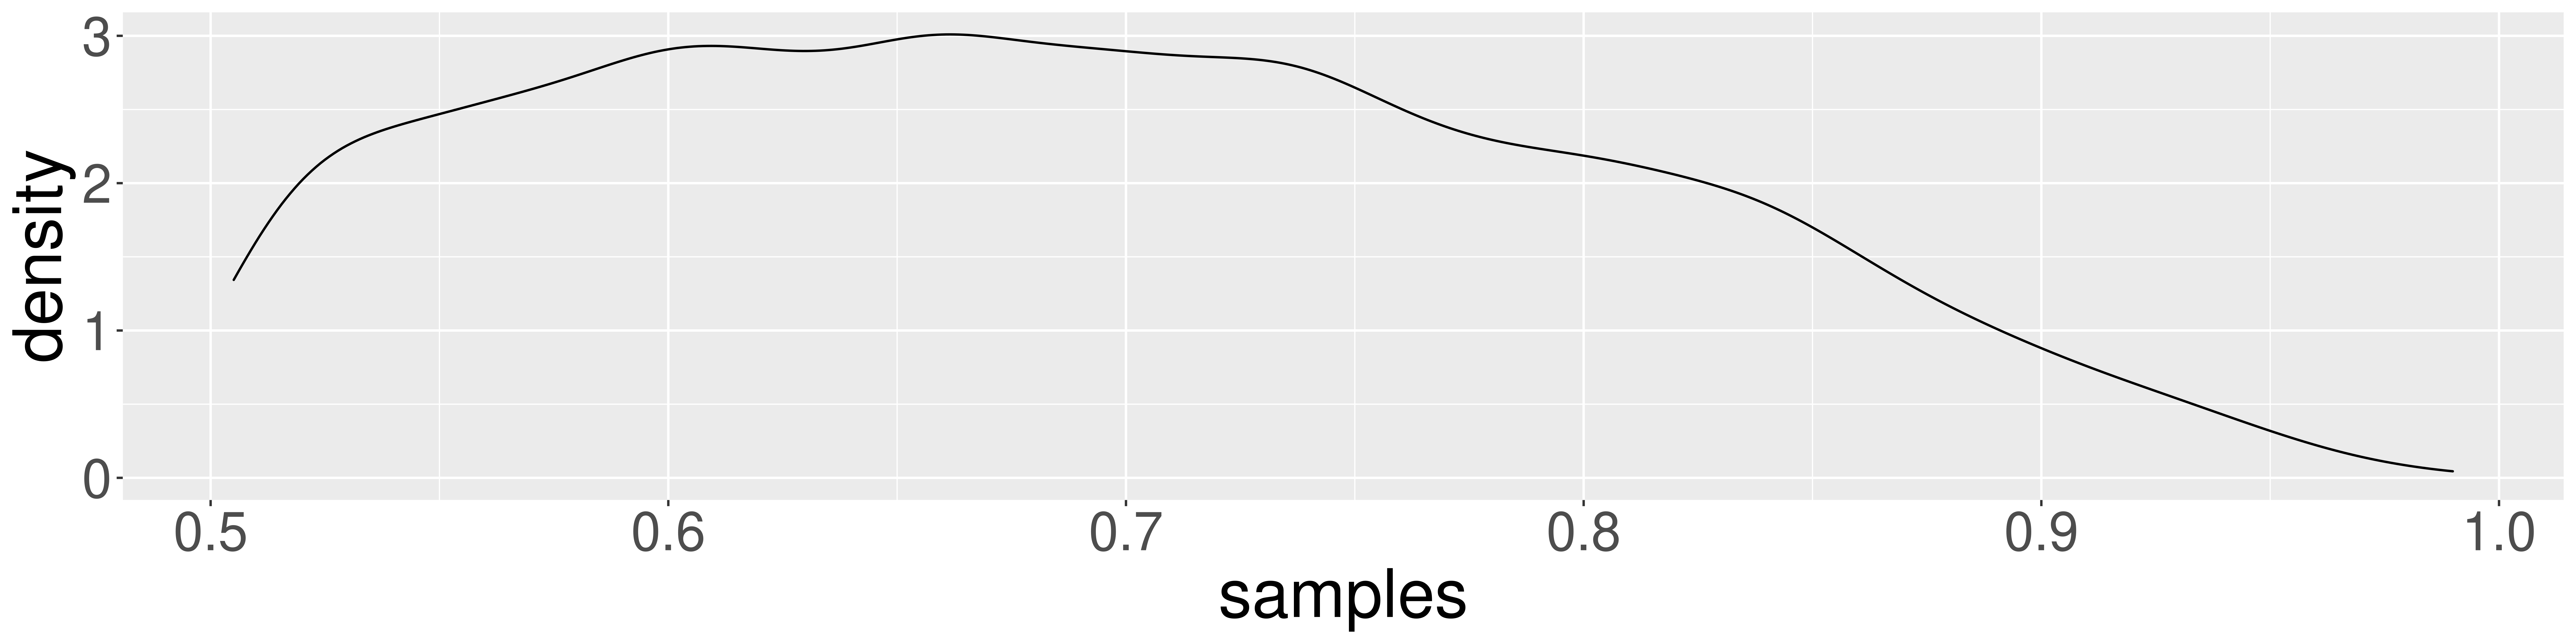
\includegraphics[width=0.8\linewidth]{figs/ex03samples.png}
\end{center}
\caption{Density of samples drawn from the posterior distribution of~\autoref{fig:ex02}.}\label{fig:ex3samples}
\end{figure}

From the samples drawn from the posterior distribution, we calculate the 89\% percentile and HPDI interval with the functions \texttt{rethinking::PI} and \texttt{rethin\hyp{}king::hpdi}.

\lstinputlisting[firstline=10, lastline=19, caption=Calculating the 89\% percentile and HPDI intervals of the samples in~\autoref{fig:ex3samples}.]{code/ex03.R}

This way, the 89\% percentile interval is described in~\autoref{tab:percentile}, and the percentile width is 0.35, as shown in~\autoref{fig:ex03a}; and the 89\% HPDI interval is described in~\autoref{tab:hpdi}, and the hpdi width is 0.35, as shown in~\autoref{fig:ex03b}.
The percentile interval has a higher width than that of HPDI\@.
This is due to the fact of the percentile interval attributing even weights for every $p$ while capturing the central 89\% probability, whereas the HPDI finds the densest interval in the distribution by searching the narrowest possible interval with the highest density.

\begin{table}[!ht]
\begin{minipage}[b]{0.42\linewidth}
\centering
\begin{tabular}{lr}
\toprule
5\% & 94\%\\
\midrule
0.5252525 & 0.8787879\\
\bottomrule
\end{tabular}
\caption{89\% percentile interval}\label{tab:percentile}
\end{minipage}
\hspace{0.1\linewidth}
\begin{minipage}[b]{0.42\linewidth}
\centering
\begin{tabular}{lr}
\toprule
|0.89 & 0.89|\\
\midrule
0.5050505 & 0.8383838\\
\bottomrule
\end{tabular}
\caption{89\% HPDI interval}\label{tab:hpdi}
\end{minipage}
\end{table}

\begin{figure}[!ht]
\begin{minipage}[b]{0.42\linewidth}
\begin{center}
  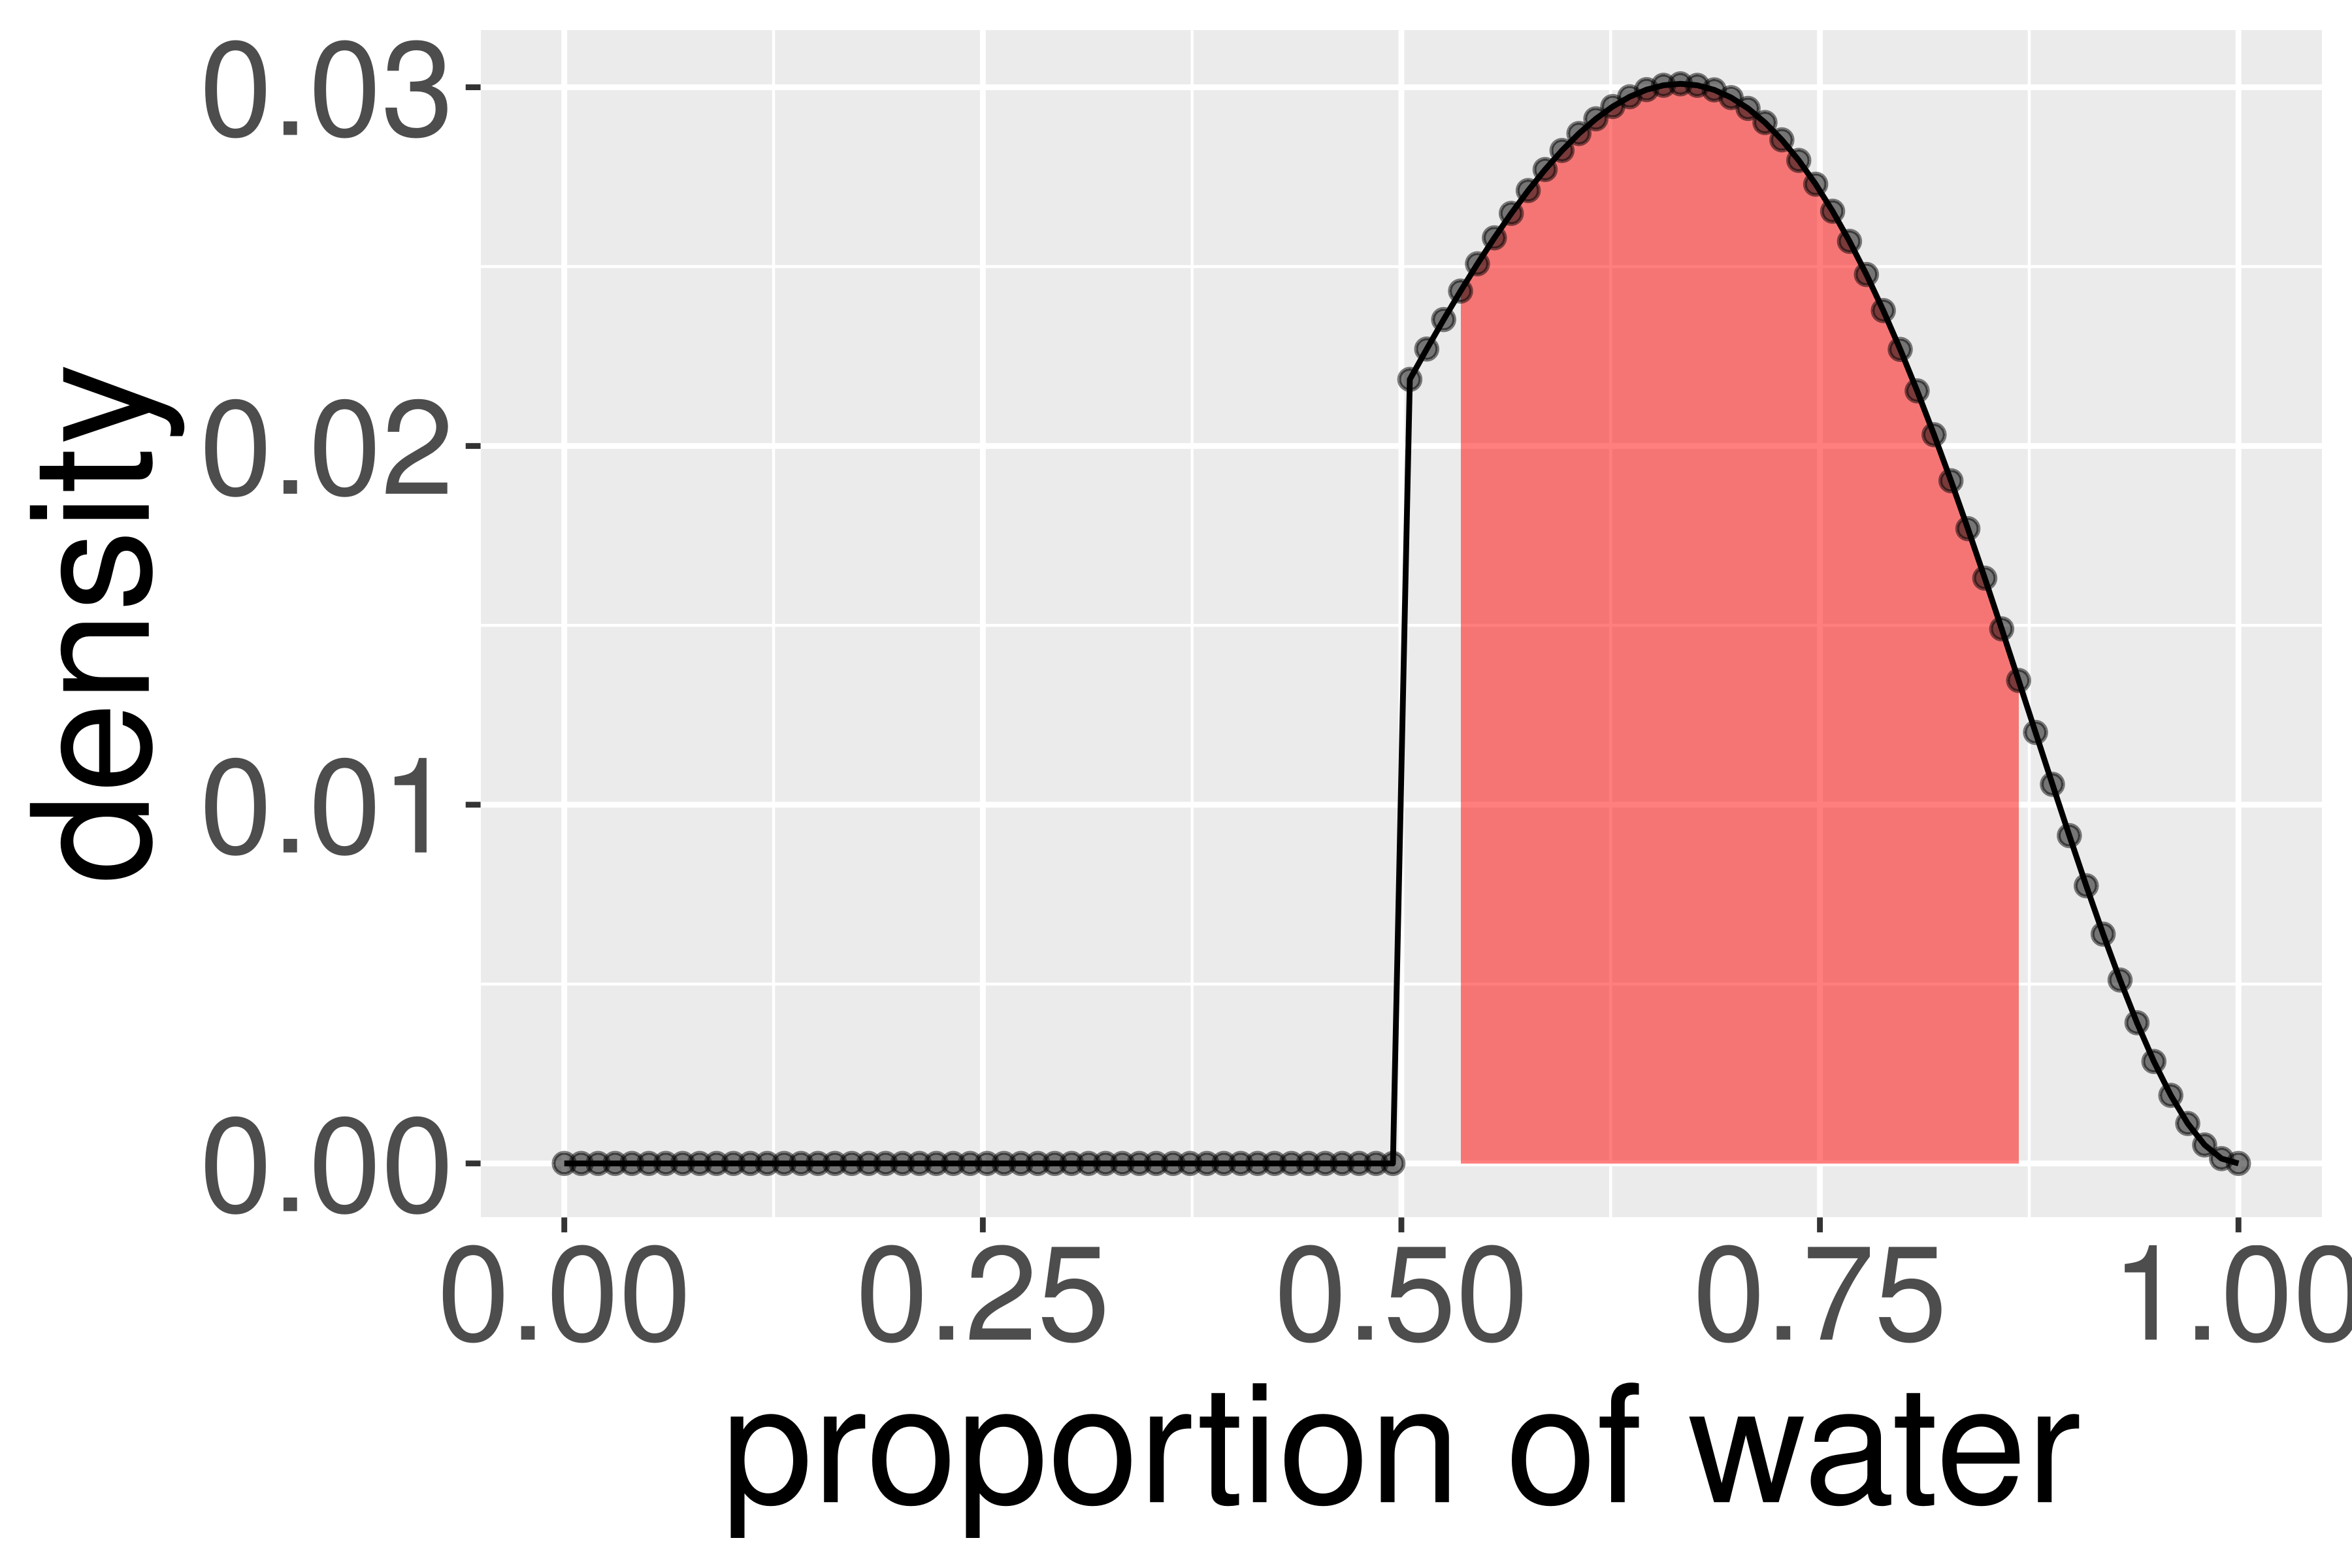
\includegraphics[width=1\textwidth]{figs/ex03percentile.png}
\end{center}
\caption{89\% percentile interval of the posterior distribution resulting from~\autoref{fig:ex02}.}\label{fig:ex03a}
\end{minipage}
\hspace{0.1\linewidth}
\begin{minipage}[b]{0.42\linewidth}
\begin{center}
  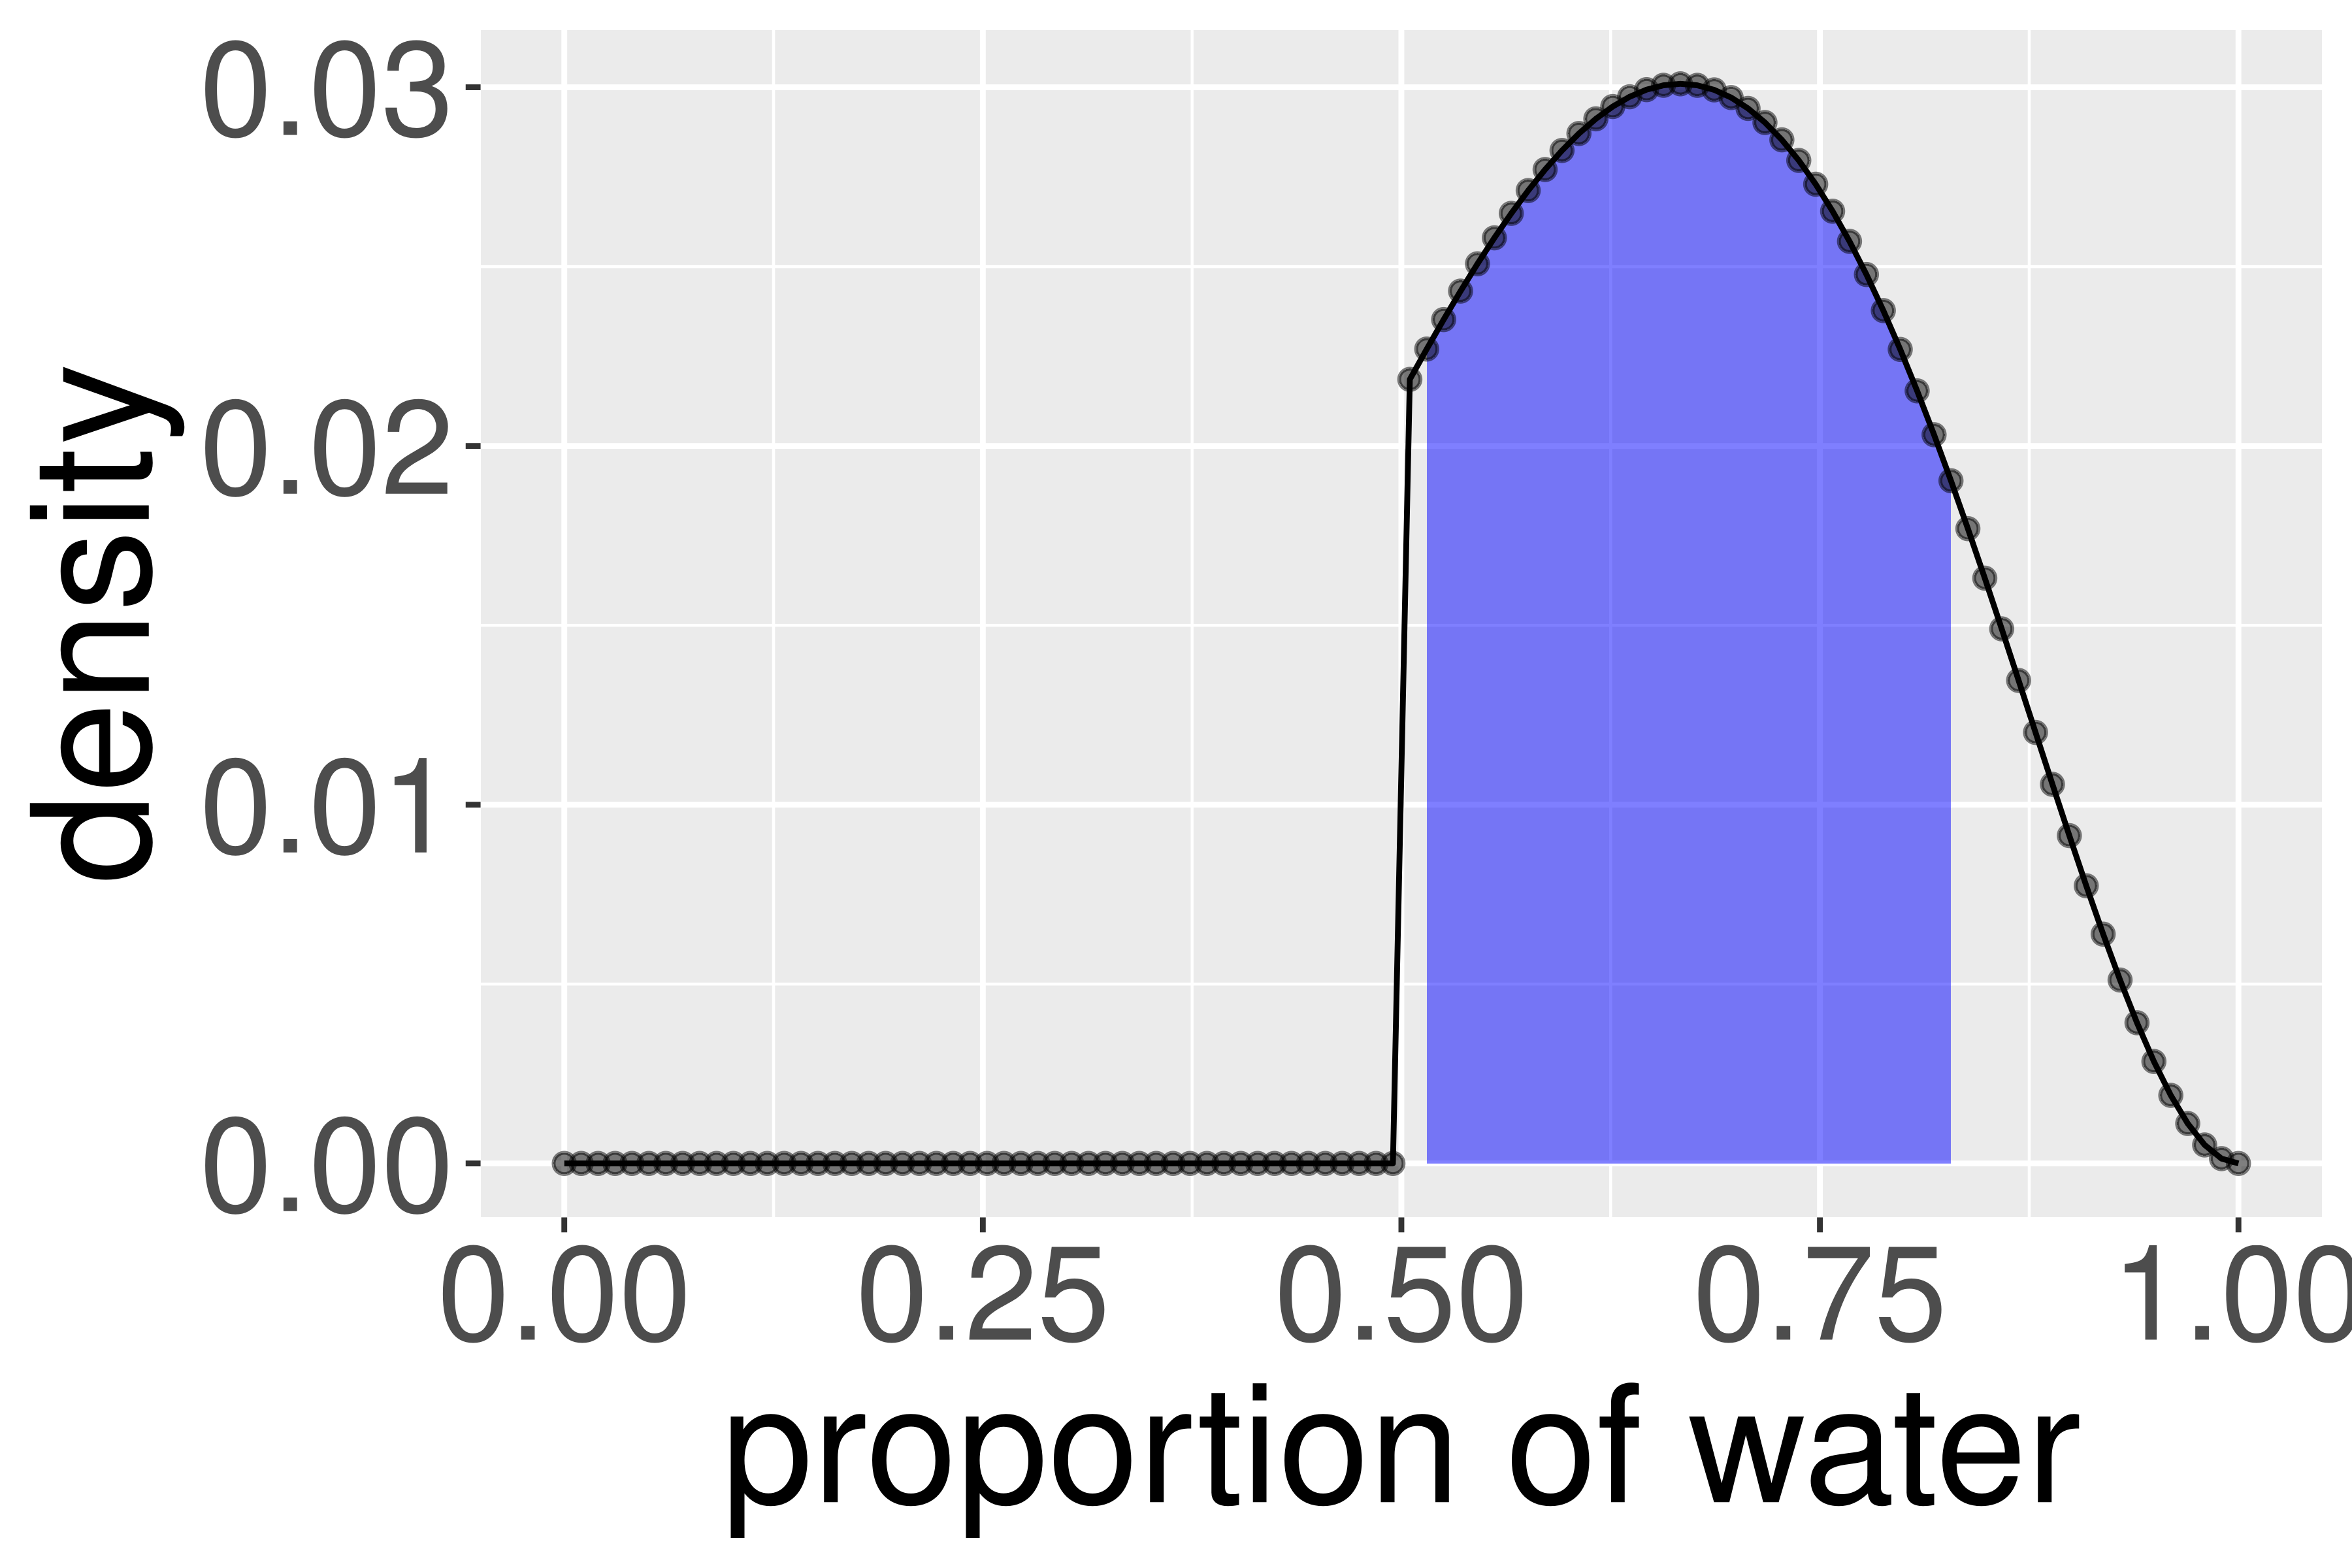
\includegraphics[width=1\textwidth]{figs/ex03hpdi.png}
\end{center}
\caption{89\% HPDI of the posterior distribution resulting from~\autoref{fig:ex02}.}\label{fig:ex03b}
\end{minipage}
\end{figure}


The intervals do not account for the region of the graph influenced by the prior distribution assumed, i.e.\ the region with 0 plausibility where the proportion of water $<$ 0.5. Without the visualization of the samples~\autoref{fig:ex3samples} and of the posterior~\autoref{fig:ex03a} and~\autoref{fig:ex03b}, it is possible to assume a less skewed posterior distribution with a much more symmetric profile.


\end{document}
